\documentclass{beamer}
\mode<presentation>
{
\usetheme{Darmstadt}
%\usecolortheme{crane} %yellow
%%% BYU colored theme
\definecolor{BYUBlue}{RGB}{00,22,55}
\definecolor{BYUTan}{RGB}{232,211,175}
\usecolortheme[named=BYUBlue]{structure}
\setbeamercolor*{palette primary}{use=structure,fg=BYUBlue,bg=lightgray}
\setbeamercolor*{palette quaternary}{fg=white,bg=lightgray!0!BYUBlue}
\setbeamercolor{frametitle}{fg=BYUBlue,bg=BYUBlue!10}
\setbeamertemplate{items}[circle]
\setbeamertemplate{blocks}[rounded][shadow=True]
\setbeamertemplate{navigations symbols}{circle}
}

\usepackage{graphics}
\usepackage[english]{babel}
\usepackage[utf8]{inputenc}
\usepackage{times}
\usepackage[T1]{fontenc}
\usepackage{array}
\usepackage{amsmath,amssymb}
\usepackage{colortbl}
\usepackage{listings}
\usepackage{tikz}
\usepackage{array}
\usepackage{threeparttable}
\usepackage{multirow}
\usepackage{amsthm}
\usepackage{float,graphicx,color}
\usepackage{graphics}
\usepackage{multicol}
\usepackage{natbib}
\usepackage{color}
\usepackage{hyperref}
\usepackage{threeparttable}
\usepackage[format=hang,font=normalsize,labelfont=bf]{caption}
\usepackage{subcaption}
\usepackage{delarray}
\usepackage{amssymb}
\usepackage{setspace}
%\usepackage[pdftex]{graphicx}
\usepackage{placeins}
\usepackage{multirow}
% \usepackage{mathtools}
\usepackage{animate}
\newcommand\ve{\varepsilon}

\title[OSPC Dynamic Scoring Model]
{OSPC Dynamic Scoring Model: \\
An Open Source Model \\ for Dynamic Revenue Estimates}

%\subtitle
%{} % (optional)

%\author%S[Author, Another] % (optional, use only with lots of authors)
%{Jason DeBacker \and Richard Evans \and Evan Magnusson \and Kerk Phillips \and Isaac Swift}
% - Use the \inst{?} command only if the authors have different
%   affiliation.

\date[Short Occasion] % (optional)
{April 1, 2015}


%\AtBeginSection[]
%{
% \begin{frame}<beamer>{Outline}
%  \tableofcontents[currentsection]
%  %\tableofcontents[currentsection, subsection]
% \end{frame}
%}

% \beamerdefaultoverlayspecification{<+->}

\begin{document}

\begin{frame}
  \titlepage
\end{frame}


\section{Overview}

  \begin{frame}
    \frametitle{Overview of the Model}
    \begin{itemize}
      \item Households
        \begin{itemize}
          \item forward looking
          \item Live up to 100 periods
          \item endogenous labor supply and savings decisions
        \end{itemize}
      \vspace{3mm}
      \item Firms
        \begin{itemize}
          \item fully dynamic
          \item endogenous investment and financial policy
        \end{itemize}
      \vspace{3mm}
      \item Government
        \begin{itemize}
          \item taxes, transfers, production of public and private goods, can run deficits
        \end{itemize}
      \vspace{3mm}
      \item Rest of world: TBD (currently closed economy)
    \end{itemize}
  \end{frame}


  \begin{frame}
    \frametitle{What's unique?}
    \begin{itemize}
      \item 100-period lived households (80 working periods)
      \vspace{2mm}
      \item Rich population dynamics (fertility, mortality, immigration)
      \vspace{2mm}
      \item Multiple treatments of bequests
      \vspace{2mm}
      \item Large set of production industries
      \vspace{2mm}
      \item Multiple assumptions about government budget balance
      \vspace{2mm}
      \item Nonlinear solution of steady-state and transition path
      \vspace{2mm}
      \item Integration of the microsimulation model
      \vspace{2mm}
      \item Open source
    \end{itemize}
  \end{frame}

    \begin{frame}
    \frametitle{Household Sector}
    \begin{itemize}
      \item OLG model with 100-period-lived agents
      \item Realistic Demographics: Fertility, Immigration, Mortality
      \item Realistic Earnings Ability Calibration
      \item Households Leave Intentional and Unintentional Bequests
    \end{itemize}
  \end{frame}


      \begin{frame}
    \frametitle{Production Sector}
    \begin{itemize}
      \item Infinitely lived, representative firms for each production industry
      \item Firms finance investment with debt, equity, and retained earnings
      \item Price of capital varies across production industry
    \end{itemize}
  \end{frame}

   \begin{frame}
    \frametitle{Model Dimensions}
    \begin{itemize}
      \item Households:
      		\begin{itemize}
		\item 80 years of economic life
		\item 7 lifetime income groups
		\item 17 consumption goods
		\end{itemize}
      \item Firms:
      	\begin{itemize}
	\item 24 production industries
	\item Corporate and non-corporate sectors in most industries
	\end{itemize}
    \end{itemize}
  \end{frame}

   \begin{frame}
    \frametitle{Consumption Goods}
% Table generated by Excel2LaTeX from sheet 'ConsumptionGoodsCategories'
\begin{table}[htbp]
  \centering
  \footnotesize
  %\caption{Add caption}
    \begin{tabular}{ll}
    \hline
    \hline
          & Consumption Good Category \\
    \hline
    1     & Food  \\
    2     & Alcohol \\
    3     & Tobacco \\
    4     & Household fuels and utilities \\
    5     & Shelter \\
    6     & Furnishings \\
    7     & Applicances \\
    8     & Apparel \\
    9     & Public transportation \\
    10    & New and used cars, fees, and maintenance \\
    11    & Cash contributions and personal care (personal services) \\
    12    & Financial services \\
    13    & Reading and entertrainment (recreation) \\
    14    & Household operations (nondurables) \\
    15    & Gasoline and motor oil \\
    16    & Health care \\
    17    & Education \\
    \hline
    \hline
    \end{tabular}%
  \label{tab:addlabel}%
\end{table}%
  \end{frame}

    \begin{frame}
    \frametitle{Production Industries}
% Table generated by Excel2LaTeX from sheet 'ProductionIndustries'
\begin{table}[htbp]
  \centering
  \tiny
  %\caption{Add caption}
    \begin{tabular}{lll}
    \hline
    \hline
    Industry Number & NAICS Code & Industry \\
    \hline
    1     & 11    & Agriculture, Forestry, Fishing and Hunting \\
    2     & 211   & Oil and Gas Extraction \\
    3     & 212 and 213 & Mining and Support Activities for Mining \\
    4     & 22    & Utilities \\
    5     & 23    & Construction \\
    6     & 32411 & Petroleum Refineries \\
    7     & 336   & Transportation Equipment Manufacturing \\
    8     & 3391  & Medical Equipment and Supplies Manufacturing \\
    9     & Other codes in 31-33 & Manufacturing \\
    10    & 42    & Wholesale Trade \\
    11    & 44-45 & Retail Trade \\
    12    & 48-49 & Transportation and Warehousing \\
    13    & 51    & Information \\
    14    & 52    & Finance and Insurance \\
    15    & 53    & Real Estate and Rental and Leasing \\
    16    & 54    & Professional, Scientific, and Technical Services \\
    17    & 55    & Management of Companies and Enterprises \\
    18    & 56    & Administrative and Support \\
    19    & 61    & Educational Services \\
    20    & 62    & Health Care and Social Assistance \\
    21    & 71    & Arts, Entertainment, and Recreation \\
    22    & 72    & Accommodation and Food Services \\
    23    & 81    & Other Services (except Government Enterprise) \\
    24    & 92    & Government Enterprise \\
    \hline
    \hline
    \end{tabular}%
  \label{tab:addlabel}%
\end{table}%
\end{frame}


\section{Households}
  \begin{frame}{Population Dynamics}\label{Population}
    New cohort every year. \\
    Becomes economically active at age E=20. \\
    Immigration and mortality over time.
    \begin{align}
      \omega_{1,t+1} &= \sum_{s=1}^{E+S} f_s\omega_{s,t}\quad\forall t \nonumber\\
      \omega_{s+1,t+1} &= (1 + i_s - \rho_s)\omega_{s,t}\quad\forall t, 1\leq s \leq E+S-1 \nonumber \\
      N_t & \equiv\sum_{s=E}^{E+S} \omega_{s,t} \quad\forall t \nonumber
    \end{align}
    \hyperlink{demographics}{\beamergotobutton{demographics}}
  \end{frame}

  \begin{frame}{Population Dynamics -- Population Distribution}
  Initial and Steady State Population Distributions by Age
  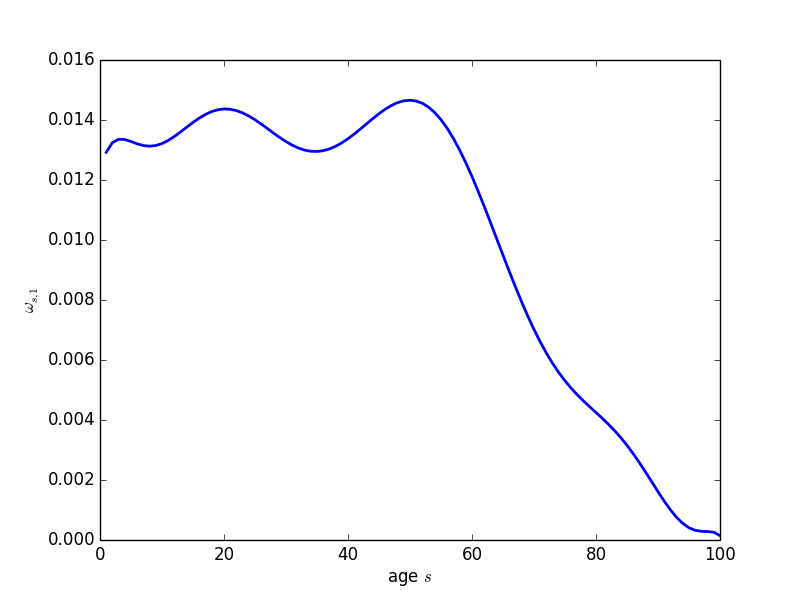
\includegraphics[scale=.275]{images/omega_init.png}
  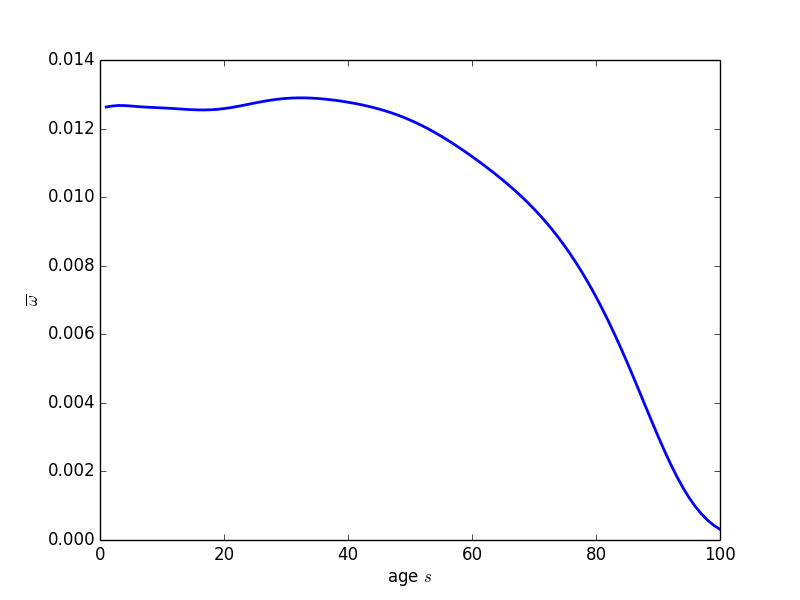
\includegraphics[scale=.275]{images/omega_ss.png}
  \end{frame}


 \begin{frame}{Summary of the Consumer's Problem}
 \label{hh_summary}
%\caption{\label{fig:hh_tree}\textbf{Summary of the Individual Problem}}
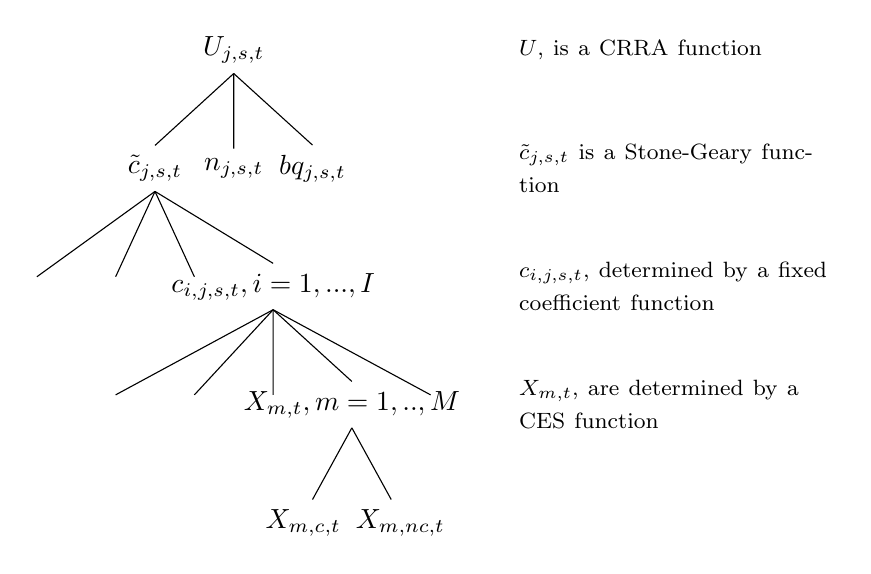
\begin{tikzpicture}
\tikzstyle{every node}=[auto,every node/.style={rectangle,draw,text centered, text width=1.3cm,minimum height=0.8cm },node distance=3cm]
\tikzset{%
level 1/.style={sibling distance = 1cm, level distance=1.5cm,edge from parent path={(\tikzparentnode.south) -- (\tikzchildnode.north)}},
level 2/.style={sibling distance = 1cm,level distance=1.5cm}
}
  \node (0){$U_{j,s,t}$}
    child {node (1) {$\tilde{c}_{j,s,t}$}
    child {node {}}
    child {node {}}
    child {node {}}
    child {node (2){$c_{i,j,s,t}, i=1,...,I$}   
child {node (3) {}}
            child {node {}}
            child {node {}}
            child {node {$X_{m,t}, m=1,..,M$}       
             child {node {$X_{m,c,t} \ \ $}}
             child {node {$\ \ X_{m,nc,t}$}}}
             child {node {}}
                        }
                  }
child {node {$n_{j,s,t}$}}
child {node {$bq_{j,s,t}$}} ;

\node at (0) [xshift=+3.5cm,right,draw=none, text width=4cm]{\footnotesize $U$, is a CRRA function };
\node at (1) [xshift=+4.5cm, right,draw=none, text width=4cm]{\footnotesize $\tilde{c}_{j,s,t}$ is a Stone-Geary function};
\node at (2) [xshift=+3.0cm, right,draw=none, text width=4cm]{\footnotesize $c_{i,j,s,t}$, determined by a fixed coefficient function };
\node at (3) [xshift=+5.0cm, right,draw=none, text width=4cm]{\footnotesize $X_{m,t}$, are determined by a CES function};
\end{tikzpicture}
\end{frame}
 

  \begin{frame}{Households -- Utility Function}\label{Utility Function}
    Utility from Consumption, Leisure and Bequests \\
    Mortality Risk;  Leisure Utility Weights Vary by Age
    \begin{equation}
      \begin{split}
        U_{j,s,t} \\
        = & \sum_{u=0}^{E+S-s}\beta^u\left[\prod_{v=s-1}^{s+u-1}(1-\rho_v)\right] u\left(c_{j,s+u,t+u},n_{j,s+u,t+u},b_{j,s+u+1,t+u+1}\right) \nonumber \\
      \end{split}
    \end{equation}
    \begin{equation}
      \begin{split}
        & u\left(c_{j,s,t},n_{j,s,t},b_{j,s+1,t+1}\right) = \frac{\left(c_{j,s,t}\right)^{1-\sigma} - 1}{1-\sigma} \\
        + & e^{g_y t(1-\sigma)}\chi^n_s\left(b\left[1 - \left(\frac{n_{j,s,t}}{\tilde{l}}\right)^\upsilon\right]^\frac{1}{\upsilon} + k\right) \\
        + & \rho_s\chi^b\frac{\left(b_{j,s+1,t+1}\right)^{1-\sigma} - 1}{1-\sigma} \nonumber \\
      \end{split}
    \end{equation}
    \hyperlink{elliptic}{\beamergotobutton{elliptic}}
  \end{frame}

  \begin{frame}
    \frametitle{Households -- Budget Constraint}
    Sources: Labor and Capital Income, Bequests \\
    Uses: Consumption, Savings and Taxes
    \begin{equation}
      \begin{split}
        & c_{j,s,t} + b_{j,s+1,t+1} + T_{j,s,t} \leq  w_t e_{j,s}n_{j,s,t} + \left(1 + r_t\right) b_{j,s,t} + \frac{BQ_{j,t}}{\lambda_jN_t}  \\
        & b_{j,1,t} = 0  \nonumber
      \end{split}
    \end{equation}
    \begin{equation}
      BQ_{j,t+1} = (1+r_{t+1})\lambda_j\left(\sum_{s=E+1}^{E+S}\rho_s\omega_{s,t}b_{j,s+1,t+1}\right) \quad\forall j,t \nonumber
    \end{equation}
  \end{frame}

  \begin{frame}{Households -- Earnings Abilities}
      Seven ability groups:
      \begin{itemize}
      \item Top 1\%
      \item Top 2-10\%
      \item Top 11-20\%
      \item Top 21-30\%
      \item Top 31-50\%
      \item Top 51-75\%
      \item Bottom 25\%
      \end{itemize}
  \end{frame}

  \begin{frame}{Households -- Earnings Abilities}
      \begin{figure}[htb]\centering
         \caption{Log of Earnings Abilities by Age and Type}
         \fbox{\resizebox{3.0in}{2.25in}{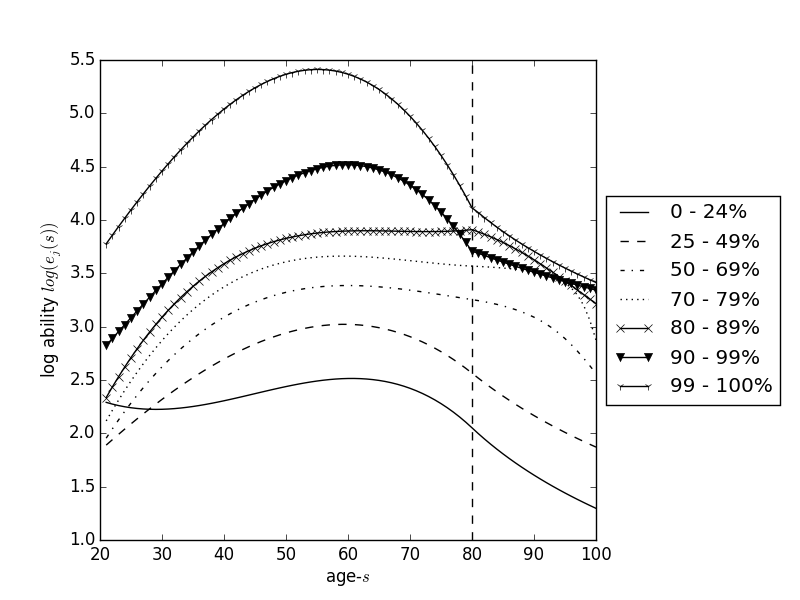
\includegraphics{images/ability_log_2D.png}}} \\
         \tiny{Data: 2013 IRS data fitted}
      \end{figure}
  \end{frame}

  \begin{frame}{Households -- Tax Structure}
    \begin{align}
      T^I_{j,s,t} & = \tau^I(\hat{a}_{j,s,t})a_{j,s,t} \nonumber \\
      & \quad\text{where}\quad \hat{a}_{j,s,t}\equiv\frac{a_{j,s,t}}{e^{g_y t}} \quad\text{and}\quad a_{j,s,t} \equiv (r_t b_{j,s,t} + w_t e_{j,s}n_{j,s,t}) \nonumber \\
      T^P_{j,s,t} & =
        \begin{cases}
          \tau^P w_t e_{j,s}n_{j,s,t} \quad\quad\quad\quad\quad\:\:\text{if}\quad s<R \\
          \tau^P w_t e_{j,s}n_{j,s,t} - \theta_j w_t \quad\quad\quad\text{if}\quad s\geq R
        \end{cases}  \nonumber \\
      T^{BQ}_{j,t} & = \tau^{BQ} \frac{BQ_{j,t}}{\lambda_j\tilde{N}_t}  \nonumber \\
      T^W_{j,s,t} & = \tau^W(\hat b_{j,s,t}) b_{j,s,t},\quad\text{where}\quad \hat{b}_{j,s,t}\equiv\frac{b_{j,s,t}}{e^{g_y t}}  \nonumber \\
      T_{j,s,t} & = T^I_{j,s,t} + T^P_{j,s,t} + T^{BQ}_{j,t} + T^W_{j,s,t} - T^L_{t} \nonumber
    \end{align}
  \end{frame}

    \begin{frame}
    \frametitle{Households -- Tax Structure}
      \begin{itemize}
      \item These functions are fit using micro data on tax burden
      \item Micro data come from the OSPC microsimulation model
      \item We integrate the two
      	\begin{itemize}
	\item Micro output results of macro forecast
	\item The macro forecast a result of tax functions
	\item Tax functions estimated from micro output
	\item A fixed point
	\end{itemize}
      \end{itemize}
  \end{frame}

  \begin{frame}{Households -- Income Tax}\label{Income Tax}
    Log scale versus normal scale
    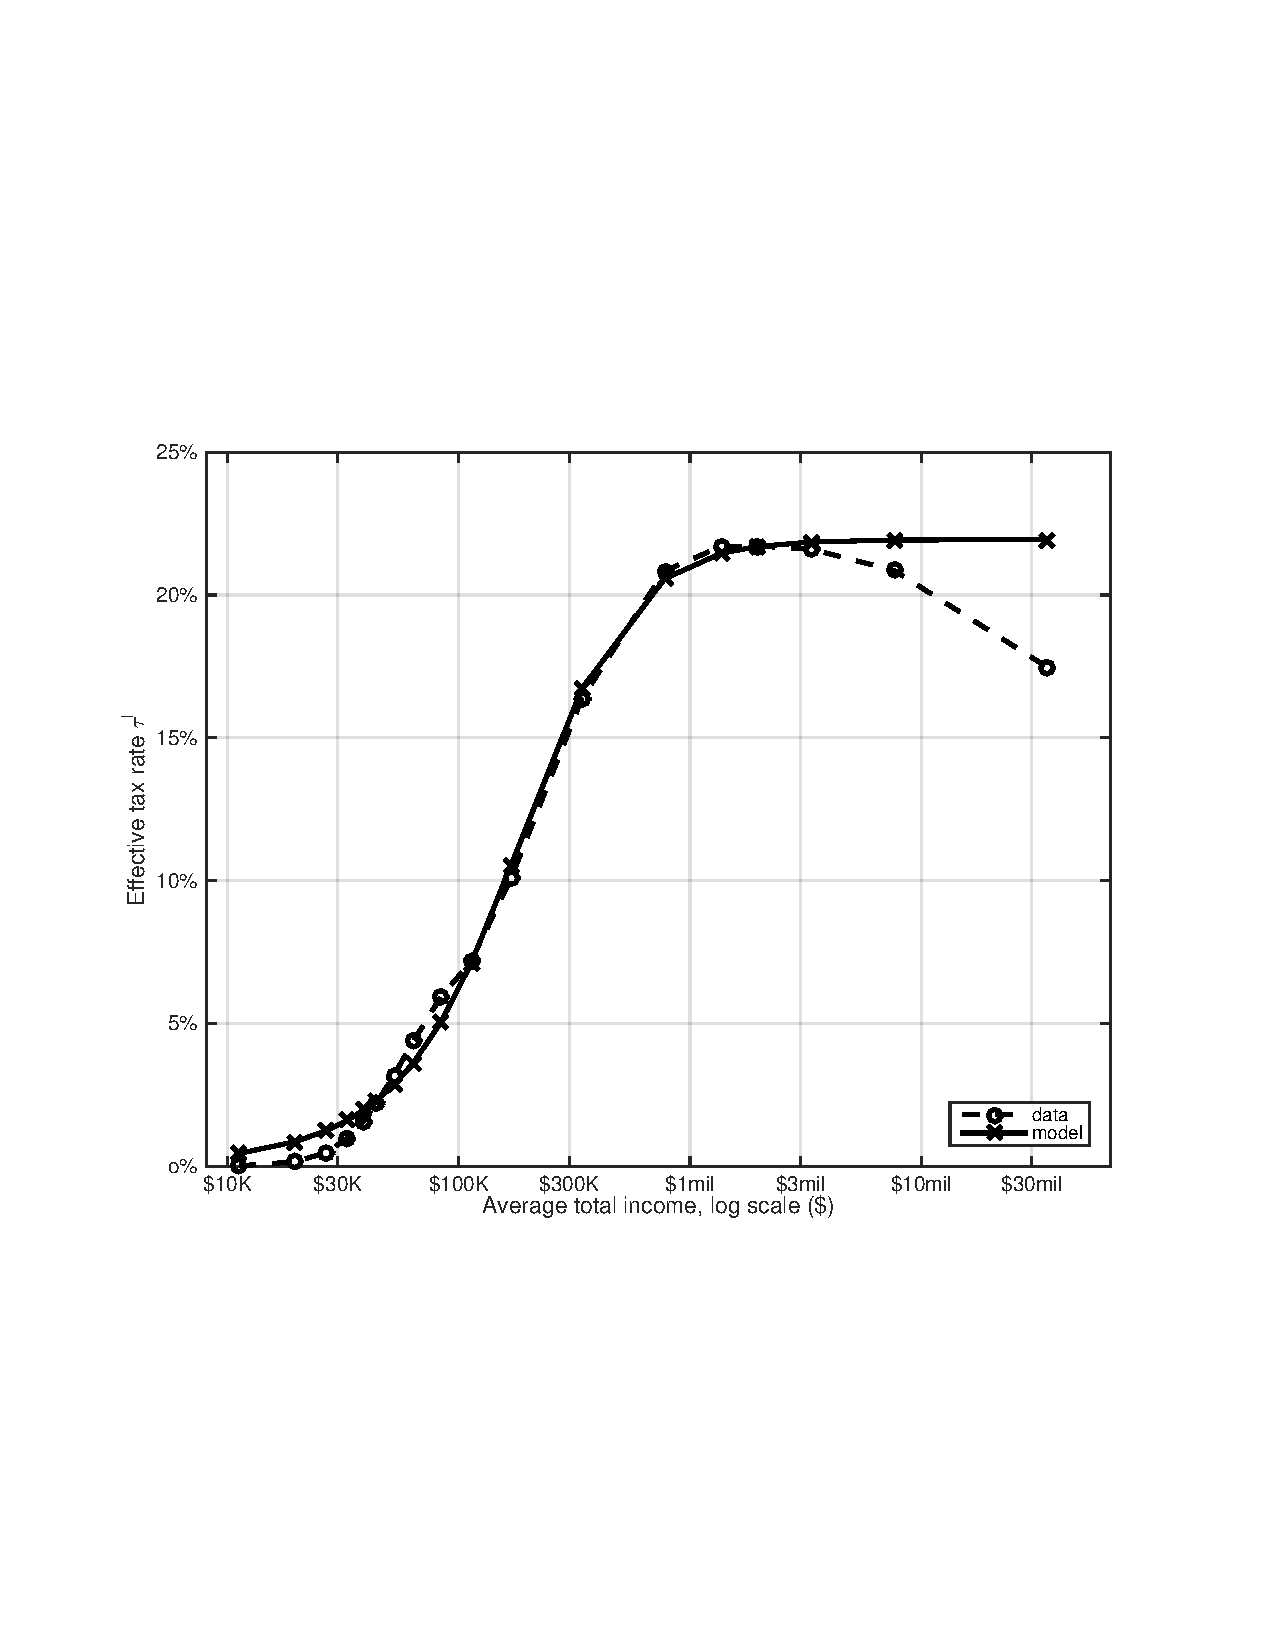
\includegraphics[scale=.275]{images/EffTaxLog.pdf}
    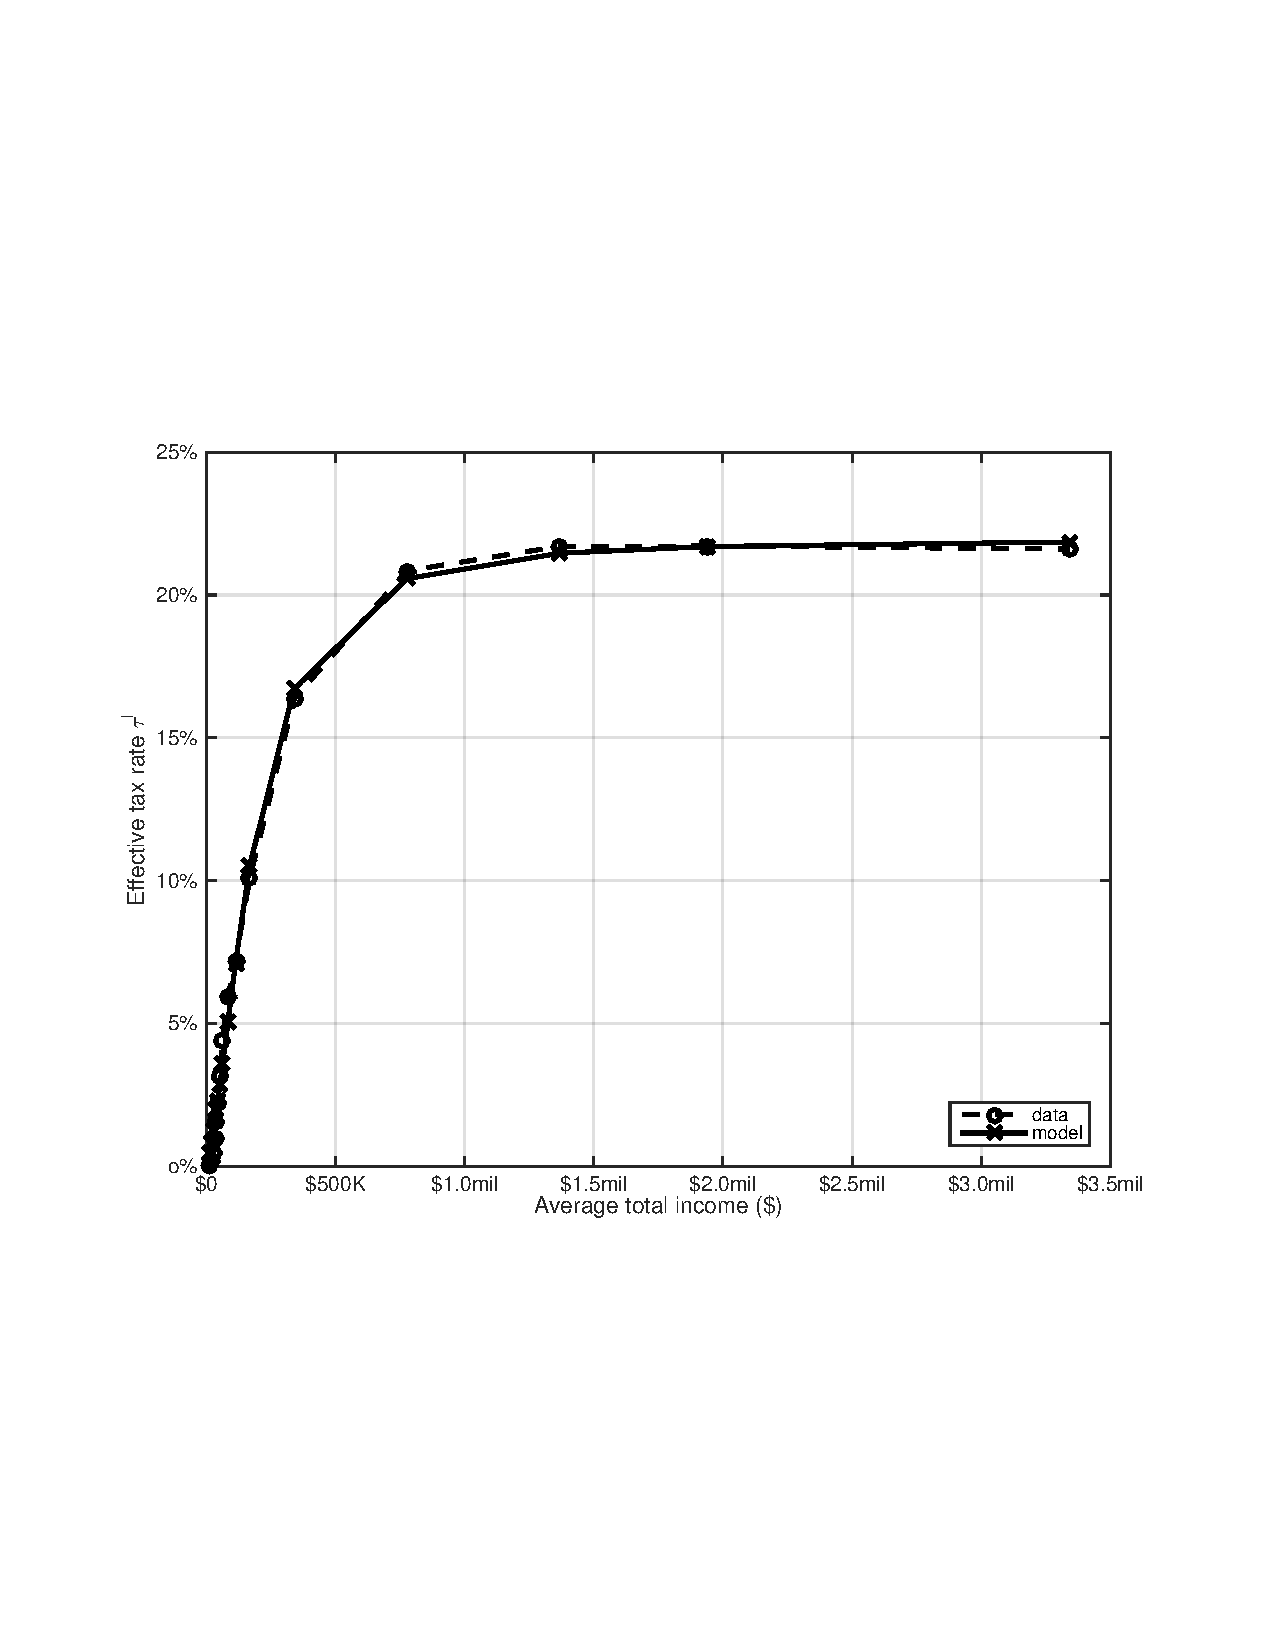
\includegraphics[scale=.275]{images/EffTaxNoLog.pdf}
  \end{frame}

\section{Firms}
  \begin{frame}{Firms -- Objective}
  Maximize Firm Value: \\
  \begin{equation}
         V_{t}= \max_{\{I_{u},EL_{u}\}^{\infty}_{u=t}}  \sum_{u=t}^{\infty} \prod_{\nu=t}^{u}\left(\frac{1}{1+\theta_{\nu}}\right)\left[ \left(\frac{1-\tau^{d}_{u}}{1-\tau^{g}_{u}}\right)DIV_{u}-VN_{u}\right]\
  \end{equation}
  \end{frame}
  
    \begin{frame}{Firms -- Taxes}
  \begin{equation}
\label{eqn:corp_tax}
\begin{split}
TE_{t}=  \tau^{b}_{t} & \left[  p_{t}X_{t}-w_{t}EL_{t}-f_{e}p^{K}_{t}I_{t}-\Phi_{t}I_{t}-f_{i}i_{t}B_{t}-f_{p}\delta b K_{t}+... \right. \\
 &  \left.  f_{b}bp^{K}_{t}I_{t}-f_{d}\delta^{\tau}K^{\tau}_{t}-\tau^{p}_{t}K_{t}\right] +\tau^{ic}_{t}p^{K}_{t}I_{t}
\end{split}
\end{equation}
 \end{frame}



\section{Government}
  \begin{frame}{Government Budget:}
  \begin{equation}
 \label{eqn:gbc}
      D_{t+1} + T^{\tau}_{t} = (1+r_{t})D_{t} + T^{H}_{t} + G^{subs}_{t} + G^{emp}_{t} + I^{G}_{t}
      \end{equation}
  \end{frame}

\section{Solution and Simulation}
  \begin{frame}{Stationarizing the Model}
    \begin{table}[htbp] \centering \captionsetup{width=3.3in}
      \caption{\label{TabStatVars}\textbf{Stationary variable definitions}}
        \begin{threeparttable}
        \begin{tabular}{>{\small}c >{\small}c >{\small}c |>{\small}c}
          \hline\hline
          \multicolumn{3}{c}{Sources of growth} & Not \\
          & & & \\[-4mm]
          $e^{g_y t}$ & $\tilde{N}_t$ & $e^{g_y t}\tilde{N}_t$ & growing\tnote{a} \\
          \hline
          & & \\[-4mm]
          $\hat{c}_{j,s,t}\equiv\frac{c_{j,s,t}}{e^{g_y t}}$ & $\hat{\omega}_{s,t}\equiv\frac{\omega_{s,t}}{\tilde{N}_t}$ & $\hat{Y}_t\equiv\frac{Y_t}{e^{g_y t}\tilde{N}_t}$ & $n_{j,s,t}$ \\[2mm]
          $\hat{b}_{j,s,t}\equiv\frac{b_{j,s,t}}{e^{g_y t}}$ & $\hat{L}_t\equiv\frac{L_t}{\tilde{N}_t}$ & $\hat{K}_t\equiv\frac{K_t}{e^{g_y t}\tilde{N}_t}$ & $r_t$ \\[2mm]
          $\hat{bq}_{j,s,t}\equiv\frac{bq_{j,s,t}}{e^{g_y t}}$ &  & $\hat{BQ}_{j,t}\equiv\frac{BQ_{j,t}}{e^{g_y t}\tilde{N}_t}$ &  \\[2mm]
          $\hat{w}_t\equiv\frac{w_t}{e^{g_y t}}$ &  &  &  \\[2mm]
          $\hat{y}_{j,s,t}\equiv\frac{y_{j,s,t}}{e^{g_y t}}$ &  &  &  \\[2mm]
          \hline\hline
        \end{tabular}
        \begin{tablenotes}
          \scriptsize{\item[a]The interest rate $r_t$ is already stationary because $Y_t$ and $K_t$ grow at the same rate. Individual labor supply $n_{j,s,t}$ is stationary.}
        \end{tablenotes}
        \end{threeparttable}
    \end{table}
  \end{frame}

  \frame{
      \frametitle{Steady-State: $2JS$ equations}
        \begin{definition}[\textbf{Stationary steady-state equilibrium}]
          A non-autarkic stationary steady-state equilibrium in the overlapping generations model with $S$-period lived agents and heterogeneous ability $e_{j,s}$ is defined as constant allocations $\hat{n}_{j,s,t}=\bar{n}_{j,s}$, $\hat{b}_{j,s+1,t+1}=\bar{b}_{j,s+1}$, and $\hat{bq}_{j,E+S+1,t+1}=\bar{bq}_{j,E+S+1}$ and constant prices $\hat{w}_t=\bar{w}$ and $\hat{r}_t=\bar{r}$ for all $j$, $s$, and $t$ such that the following conditions hold:
          \begin{enumerate}
            \item households $J$ optimize according to $2S$ Euler equations,
            \item firms $M\times 2$ optimize according to 2 FOCs,
            \item markets clear according to 3 market clearing conditions, and
            \item the population has reached its stationary steady state distribution $\bar{\omega}_s$ for all ages $s$.
          \end{enumerate}
        \end{definition}
      }


  \begin{frame}{Transition Path Solution Method}\label{TPI Solution}
    \frametitle{Stationary non-steady-state equilibrium}
      \begin{definition}[\textbf{Stationary non-steady-state equilibrium}]
        A non-autarkic stationary non-steady-state equilibrium in the overlapping generations model with $S$-period lived agents and heterogeneous ability $e_{j,s}$ is defined as allocations $n_{j,s,t}$, $\hat{b}_{j,s+1,t+1}$, and $\hat{bq}_{j,E+S+1,t+1}$ and prices $\hat{w}_t$ and $r_t$ for all $j$, $s$, and $t$ such that the following conditions hold:
        \begin{enumerate}
          \item households and firms have symmetric beliefs, $\Omega(\cdot)$, about the evolution of the distribution of savings, and those beliefs about the future distribution of savings equal the realized outcome (rational expectations),
          \item households $J$ optimize according to $2S$
          \item firms $M\times 2$ optimize according to 2 FOCs, and
          \item markets clear according to 3 market clearing conditions.
        \end{enumerate}
      \end{definition}
  \end{frame}

 


\section{Summary}

  \begin{frame}{The GitHub Repo}
  The open, online repository houses all model code, data, and documentation: \\
  \ \\
\href{https://github.com/OpenSourcePolicyCenter/dynamic}{https://github.com/OpenSourcePolicyCenter/dynamic}
  \end{frame}

  \begin{frame}{Summary}
  \begin{itemize}
      \item Detailed macro model
      \item Efficient code
      \item Year by year effects
      \item Integration with microsimulation model
  \end{itemize}
  \end{frame}


\end{document}
